\documentclass[a4paper]{fhnwreport}
\usepackage{pdfpages}

\graphicspath{{./graphics/}{./Anhang/}}	

\title{Fachbericht Virtual Sun}
\author{HS15 Pro3E Team 3}
\date{Windisch, \today}

\begin{document}

\maketitle

\vspace*{2cm}
\begin{figure}[h]
	\centering
		
\includegraphics[width=0.80\textwidth]{virtualsun-logo.jpg}
	\label{fig:virtualsun-logo}
\end{figure}
\vfill
\textsc{
\begin{tabbing}
Auftraggeber: \hspace{4em} \=   Hans Gysin \\[2ex]
Betreuer:  \> Matthias Meier (Controllerprogrammierung) \\ \> Peter Ganzmann (Analogtechnik) \\ \> Bonnie Domenghino (Englisch) \\ \> Anita Gertiser (Kommunikation) \\[2ex]
Gruppe:  \>  HS15 pro3E Team 3 \\[2ex]
Teammitglieder:  \> Simonetta Sturm (Projektleiter) \\ \> Yanick Frei \\ \> Claudius Jörg \\[2ex]
Studiengang: \> Elektro- und Informationstechnik
\end{tabbing}}
\vfill
\hbox{}
\clearpage

%\includepdf[pages=-]{Abstract.pdf}
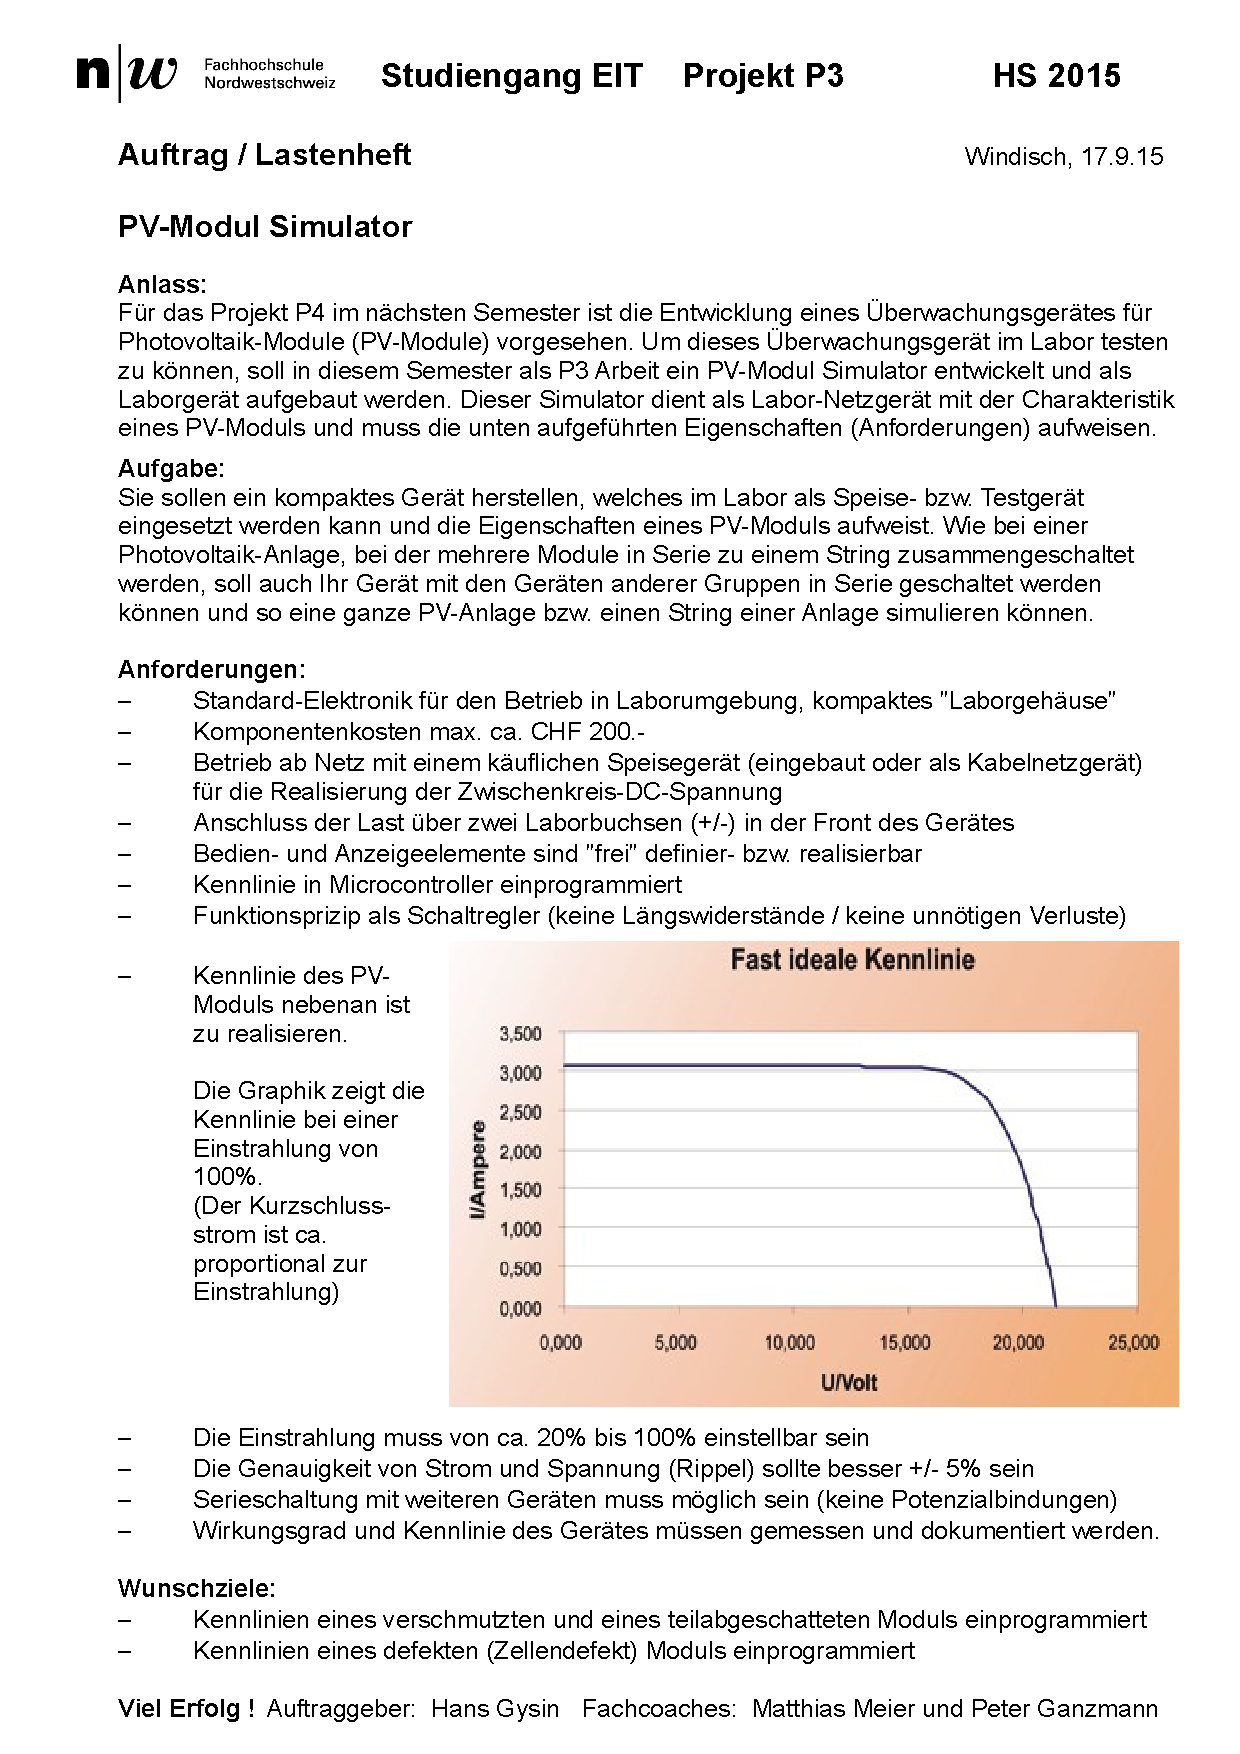
\includepdf{Lastenheft_EIT_P3_15HS.pdf} 

\tableofcontents	
\setcounter{page}{1}
\clearpage

\section{Einleitung}
\section{Theoretische Grundlagen}

\subsection{Solarzellen}
\subsection{Mathematik}

\subsubsection{Berechnung der Solarzellenkennlinie}

Gemäss \colorbox{red}{Quelle: Photovoltaik Engineering} lässt sich die Kennlinie der Solarzelle aus folgenden Parametern berechnen:
\begin{align*}
	I_{SC} &= 3.09A \\
	U_{OC} &= 22.0V \\
	I_{Pmax} &= 2.90A \\
	U_{Pmax} &= 18.0V
\label{eq:eingangsparameter_kennlinie}
\end{align*}

Mit diesen Werten können die weiteren Parameter $M$ (Steigung im Leerlaufpunkt), $R_{Pv}$ (Solarzellenwiderstand), $U_T$ (Temperaturspannung) $I_0$ (Sperrstrom) und $I_{Ph}$ (Photostrom) berechnet werden:
\begin{equation}\begin{split}
	M&=\frac{U_{OC}}{I_{SC}}\cdot\left(-5.411\cdot\frac{I_{Pmax}\cdot U_{Pmax}}{I_{SC}\cdot U_{OC}}+6.450\cdot\frac{U_{Pmax}}{U_{OC}}+3.417\cdot\frac{I_{Pmax}}{I_{SC}}-4.422\right) \\
	&=-0.6607
\label{eq:kennlinie_m}
\end{split}\end{equation}
\begin{equation}
	R_{Pv}=-M\cdot\frac{I_{SC}}{I_{Pmax}}+\frac{U_{Pmax}}{I_{Pmax}}\cdot\left(1-\frac{I_{SC}}{I_{Pmax}}\right)=0.2973\Omega
\label{eq:kennlinie_rpv}
\end{equation}
\begin{equation}
	U_T=-\left(M+R_{Pv}\right)\cdot I_{SC}=1.1228V
\label{eq:kennlinie_ut}
\end{equation}
\begin{equation}
	I_0=I_{SC}\cdot e^{\frac{U_{OC}}{U_T}}=9.5637nA
\label{eq:}
\end{equation}
\begin{equation}
	I_{Ph}=I_{SC}=3.09A
\label{eq:kennlinie_iph}
\end{equation}

Mit den Werten von (\ref{eq:kennlinie_m}) bis (\ref{eq:kennlinie_iph}) kann nun mit folgender Formel die Kennlinie der Solarzelle berechnet werden:
\begin{equation}
	U\left(I\right)=U_T\cdot\ln\left(\frac{I_{Ph}-I+I_0}{I_0}\right)-I\cdot R_{Pv}
\label{eq:kennlinie}
\end{equation}

Die Kennlinie, welche in Abbildung \ref{fig:Kennlinie} dargestellt ist, wurde aus (\ref{eq:kennlinie}) mittels Matlab erzeugt. Dazu wurde die Spannung U auf die x-Achse und der Strom I auf die y-Achse aufgetragen. Abbildung \ref{fig:Kennlinie_Lastenheft} zeigt zum Vergleich die vom Auftraggeber geforderte Kennlinie. Da zwischen den beiden Kennlinien keine Unterschiede bemerkbar sind, wird (\ref{eq:kennlinie}) als gültig betrachtet.
\begin{figure}
	\centering
		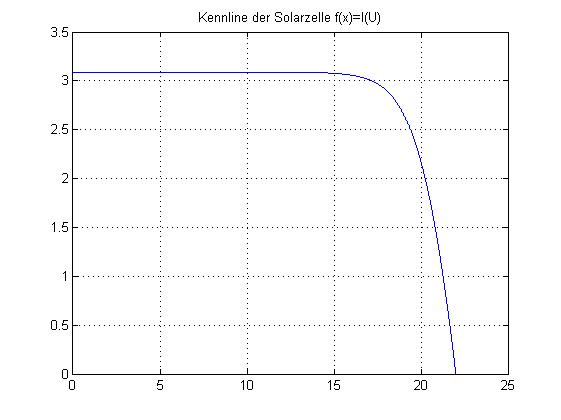
\includegraphics[width=0.9\textwidth]{Kennlinie.jpg}
	\caption{Die Kennlinie, welche mittels der Formeln ermittelt wurde.}
	\label{fig:Kennlinie}
\end{figure}
\begin{figure}
	\centering
		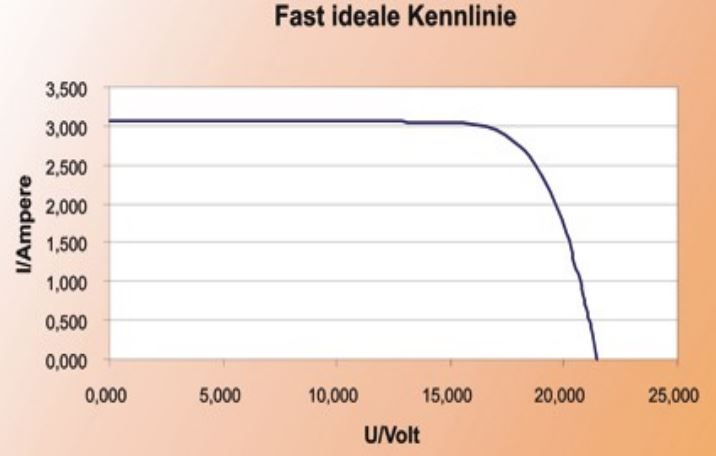
\includegraphics[width=0.60\textwidth]{Kennlinie_Lastenheft.jpg}
	\caption{Die Kennlinie, welche mittels der Formeln ermittelt wurde.}
	\label{fig:Kennlinie_Lastenheft}
\end{figure}

\subsubsection{Anpassung der Kennlinie bei verschiedenen Bestrahlungsstärken}
Gemäss dem Lastenheft soll es ausserdem möglich sein, die Bestrahlungsstärke in einem Wertebereich von 20\% bis 100\% einstellen zu können. Bei Abnahme der Bestrahlung verschiebt sich die Kennlinie nach unten, sodass der Stromwert folgendermassen angepasst werden muss:
\begin{equation}
	I_{neu}=I+\frac{100-\left[\text{Bestrahlungsstärke in Prozent}\right]}{100}\cdot I_{SC}
\label{eq:kennlinie_prozent}
\end{equation}
Beispielhaft wurden mittels Matlab zwei zusätzliche Kennlinien für 60\% und 20\% dargestellt, zu sehen in Abbildung \ref{fig:Kennlinie_Auslastung}. Die beiden Kennlinien bei verringerter Bestrahlungsstärke verhalten sich bei $I_{neu}>I_{SC}$ unerwünscht, im Programm selbst wird dies jedoch mittels einer if-Prüfung verhindert.
\begin{figure}
	\centering
		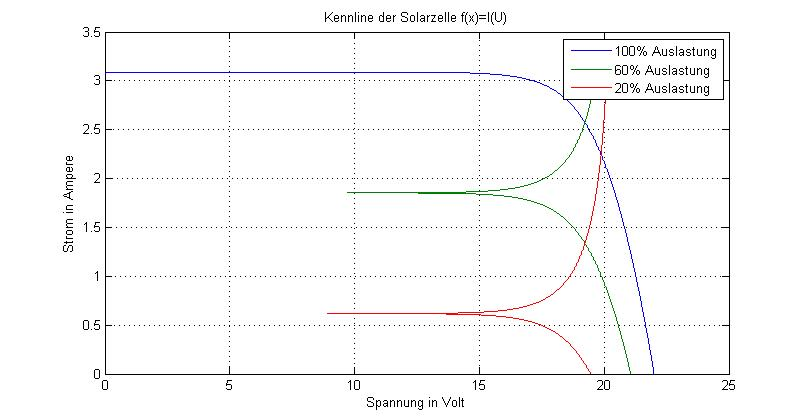
\includegraphics[width=0.9\textwidth]{Kennlinie_Auslastung.jpg}
	\caption{Verhalten der Kennlinie bei verschiedenen Bestrahlungsstärken.}
	\label{fig:Kennlinie_Auslastung}
\end{figure}

\section{Hardware}

\subsection{Controller}

Für die Auswahl des Mikrocontrollers waren folgende Punkte entscheidend:
\begin{itemize}
	\item Eingebaute Analog-Digital-Wandler zum Auslesen der Messwerte. Diese sollten mindestens eine Auflösung von 8bit, besser noch mehr besitzen.
	\item Der Programmspeicher muss genügend gross zur Aufnahme des Programmes sein. 8kByte werden als Minimum festgesetzt.
	\item Eingebaute Interfaces für SPI und I$^2$C, um mit anderen Bauteilen zu kommunizieren
	\item Genügend I/O Anschlüsse, um den Bildschirm (6 Pins), die drei Taster (3 Pins), die beiden Analog-Digital-Wandler (2 Pins) und das Interface für den Digital-Analog-Wandler (4 Pins).
	\item Eine Versorgungsspannung von 5V sollte zulässig sein, damit für den Mikrocontroller keine eigene Spannung erzeugt werden muss.
\end{itemize}

Diesen Bedingungen entspricht der ATmega328P von Atmel. Um den Aufwand für den Aufbau des Mikrocontrollers zu verringern wurde ein Arduino Uno Board gewählt. Der Arduino Uno besitzt bereits einen Oszillator für 16MHz und eine USB-Schnittstelle zur einfachen Programmierung, ausserdem sind sämtliche Pins bereits nach aussen auf Buchsenleisten geführt.

Die Analog-Digital-Wandler des ATmega328P kennen zwei Betriebsmodis: Die anliegende Spannung kann mit einer internen oder einer externen Spannungsreferenz verglichen werden. Die externe Spannungsreferenz bietet den Vorteil, dass deren Genauigkeit bekannt und höher als die interne ist. Ausserdem kann bei der externen Spannungsreferenz eine höhere Spannung, in unserem Fall 5V (intern: 1.1V), gewählt werden, was die Messung unempfindlicher gegenüber Störungen macht.
\subsection{Messschaltung}

Um die Ausgangskennlinie regeln zu können, müssen die Ausgangsgrössen Spannung (in der Software als $istU$ bezeichnet) und Strom (in der Software als $istI$ bezeichnet) bekannt sein. Die Eingänge des Mikrocontrollers können aber nur Spannungen im Bereich zwischen 0V und 5V mit einer Genauigkeit von 10bit messen. Folglich wird eine Schaltung benötigt, welchen den Spannungsbereich 0V bis 24V und den Strombereich 0A bis 3.5A jeweils auf den Spannungsbereich zwischen 0V und 5V anpassen. Im folgenden Abschnitt wird genauer auf diese Schaltung eingegangen, welche in Abbildung \ref{fig:Messschaltung} dargestellt ist.
\begin{figure}[h]
	\centering
		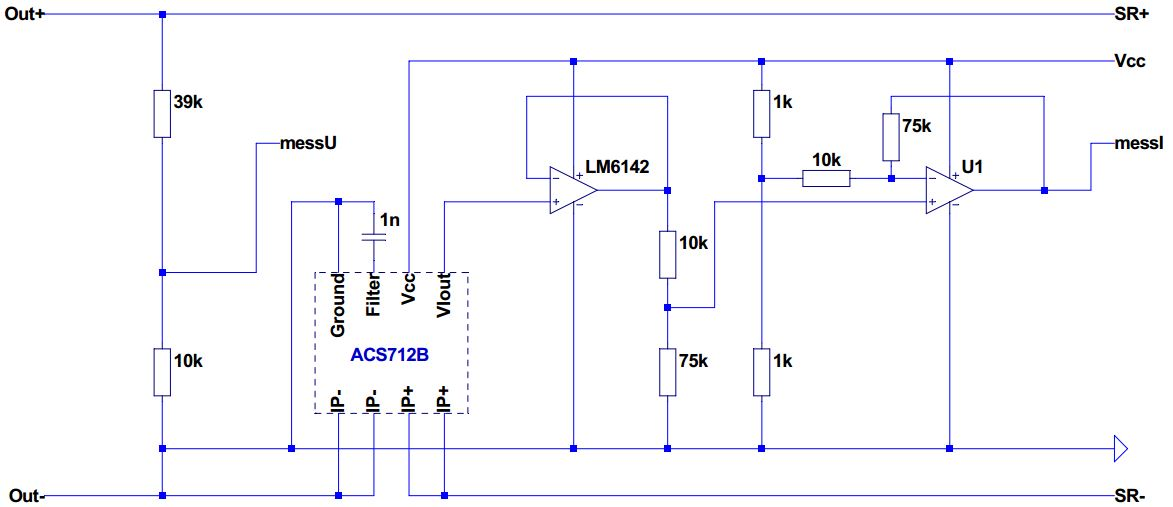
\includegraphics[width=1.00\textwidth]{Messschaltung.JPG}
	\caption{Die komplette Messschaltung.}
	\label{fig:Messschaltung}
\end{figure}


\subsubsection{Spannungsmessung}
\begin{figure}[h]
	\centering
		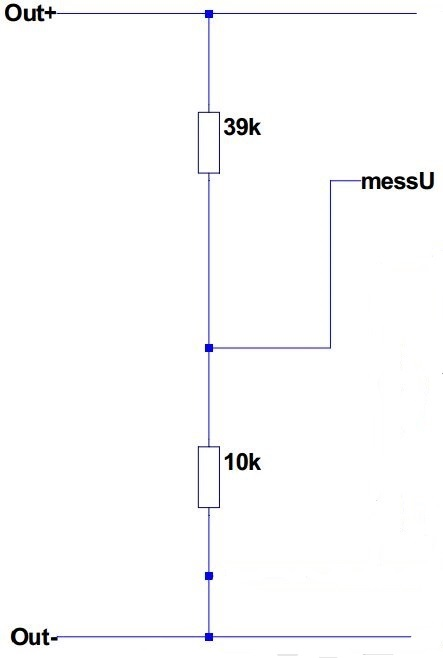
\includegraphics[width=0.30\textwidth]{Messschaltung_U.JPG}
	\caption{Die Messschaltung zur Spannungsmessung.}
	\label{fig:Messschaltung_U}
\end{figure}

Um die Spannung am Ausgang messen zu können, wird ein Spannungsteiler benötigt. Im einfachsten Fall kann ein Spannungsteiler aus zwei Widerständen bestehen, Abbildung \ref{fig:Messschaltung_U} zeigt diesen Spannungsteiler. Die Spannung $messU$ berechnet sich nach folgender Formel:
\begin{equation}
	messU=\frac{\Delta U\cdot R_2}{R_1+R_2}=\frac{U_{Out}\cdot10k\Omega}{39k\Omega +10k\Omega}=\frac{U_{Out}}{4.9}
\label{eq:messU}
\end{equation}
 Die beiden Widerstände sollten dabei folgende Bedingungen erfüllen:
\begin{itemize}
	\item Da innerhalb der Messschaltung selbst eine Spannung abfallen kann ist es wichtig, die Spannungsmessung möglichst nahe am Ausgang vorzunehmen.
	\item Um bei 24V Ausgangsspannung am Ausgang des Spannungsteiler 5V zu erhalten, sollte das Ver\-hält\-nis der Widerstände ungefähr $\frac{R_1}{R_2}=3.8$ betragen.
	\item Die Widerstände sollten nicht zu klein dimensioniert werden, um die Schaltung nicht zu belasten.
	\item Die Widerstände sollten nicht zu gross dimensioniert werden, sodass der Eingang des Mikrocontrollers die Messung nicht verfälscht.
\end{itemize}
Aus diesem Grund wurde $R_1=39k\Omega$ und $R_2=10k\Omega$ gewählt. Damit die Schaltung reproduzierbar gestaltet werden kann, wurden Metallschichtwiderstände mit einer Genauigkeit von $\pm 1\%$ verwendet. Die Genauigkeit der Schaltung wurde ausserdem mit einer Messreihe \ref{subsec_messu} auf Seite \pageref{subsec_messu} verifiziert.

\subsubsection{Strommessung}
\begin{figure}[h]
	\centering
		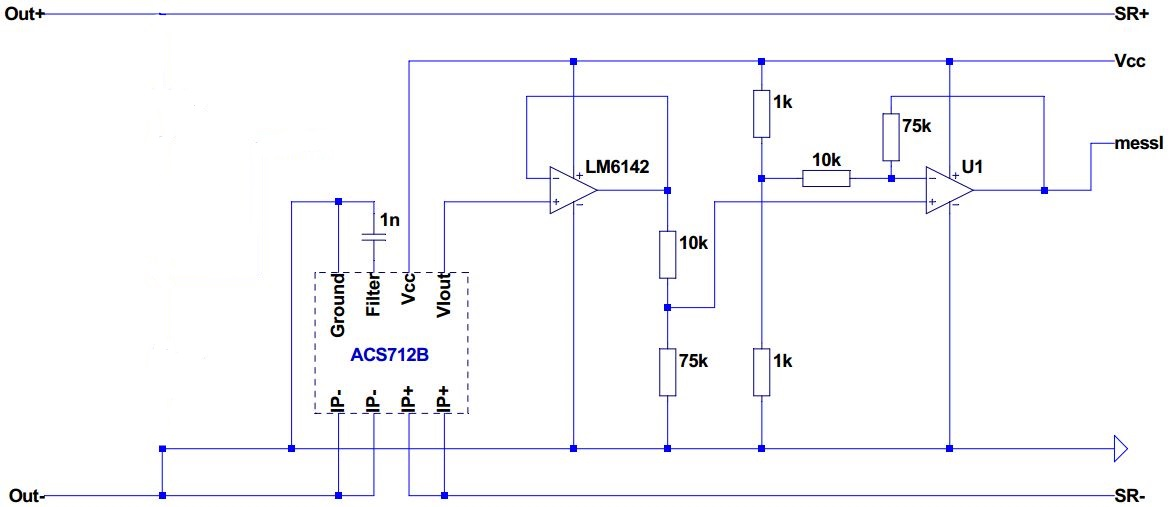
\includegraphics[width=1.00\textwidth]{Messschaltung_I.JPG}
	\caption{Die Messschaltung zur Strommessung.}
	\label{fig:Messschaltung_I}
\end{figure}
Die Messung des Stromes wird oftmals mit einem Shuntwiderstand bestimmt, über dem der Spannungsabfall gemessen wird. Da dies jedoch zwangsläufig mit Verlusten verbunden ist und ausserdem die Ausgangsspannung abhängig vom Strom verfälscht, wurde ein Hallsensor gewählt, der diese Nachteile nicht besitzt. Hallsensoren liefern eine Ausgangsspannung, die proportional zum Produkt aus magnetischer Feldstärke und Strom ist. Da die magnetische Feldstärke konstant ist, ist die Ausgangsspannung proportional zum Strom.

Der ACS712B von Allegro MicroSystems \cite{db_acs712} besitzt eine Sensitivität von 185mV/A sowie einen Spannungsoffset von Vcc/2. Diese Spannung wird, da der Ausgangswiderstand des ACS712B mit mindestens 4.7k$\Omega$ eher hoch ist, zuerst in einer Impedanzwandlerschaltung mit einem Operationsverstärker niederohmig gemacht. Bei einem Strombereich von 0A bis 3.5A wird dabei lediglich ein Spannungsbereich von 2.5V bis 1.85V ausgenutzt. Aus diesem Grund wird die Ausgangsspannung des ACS712B zuerst mit einer Subtraktionsschaltung vom Offset bereinigt, wodurch ein Spannungsbereich von -0.65V bis 0.0V entsteht. Anschliessend wird diese Spannung um den Faktor -7.5 verstärkt, sodass der Spannungsbereich des Einganges des Mikrocontrollers voll ausgenutzt werden kann. Das Bereinigen vom Offset und die Spannungsverstärkung kann mit einem einzigen Operationsverstärker umgesetzt werden. Dies bringt ausserdem den Vorteil, das keine negative Versorgungsspannung benötigt wird. Die Widerstandswerte sollten dabei nicht zu klein sein, damit die Ausgänge nicht zu sehr von den Widerständen belastet werden. Die Widerstandswerte sollten aber auch nicht zu gross sein, sodass die Schaltung genügend Strom für die Eingänge der Operationsverstärker beziehungsweise des Mikrocontrollers liefern kann.  Die theoretischen Grundlagen zu den Operationsverstärkerschaltungen können in \cite{operationsverstaerker} nachgelesen werden. Die Spannung $messI$ kann mit folgender Formel berechnet werden:
\begin{equation}
	messI=\left(\frac{Vcc}{2}-185mV\cdot I_{Out}-\frac{Vcc\cdot 1k\Omega}{1k\Omega +1k\Omega}\right)\cdot -\frac{75k\Omega}{10k\Omega}=1.3875\cdot I_{Out}
\label{eq:messI}
\end{equation}

Für diese Anpassung des Messresultates werden zwei Operationsverstärker benötigt. Die Auswahl des Operationsverstärkers erfolge nach folgenden Kriterien:
\begin{itemize}
	\item Nach Möglichkeit sollten beide Operationsverstärker in einem Gehäuse verbaut sein.
	\item Der Operationsverstärker sollte mit einer einseitigen Speisung von 5V betrieben werden können.
	\item Die Ausgangsspannung des Operationsverstärker sollte den kompletten Bereich von 0V bis 5V ausnützen können, aus diesem Grund sollte ein Rail-To-Rail Design verwendet werden.
\end{itemize}
Aus diesen Gründen wurde das Modell LM6142BIN von National Semiconductor \cite{lm6142} gewählt. Die Genauigkeit der Schaltung wurde ausserdem mit einer Messreihe \ref{subsec_messi} auf Seite \pageref{subsec_messi} verifiziert.
\documentclass[a4paper]{fhnwreport}
\usepackage{pdfpages}
%\usepackage{float}

\graphicspath{{./graphics/}{./Anhang/}}	
\begin{document}

\subsection{Schaltregler}\label{schaltregler}

Gemäss Vorgaben des Auftraggebers wurde das zur Spannungsregelung zuständige Bauteil mittels eines Abwärtswandlers im Form eines Schaltreglers realisiert. Die Ausgangsspannung des Reglers soll vom Controller in Form einer DC-Spannung reguliert, sodass der Ausgang der im Mikrocontroller Kennlinie entspricht. 

Gewählt wurde der LT1074CT, da dieser Ströme bis zu 5A sowie eine maximale Ausgangsspannung von 50V besitzt. Die maximale Eingansspannung beträgt 60V, deutlich mehr als die Spannung des Netzgerätes, welches 24V liefert.
Des weiteren lässt sich der LT1074CT mittels eines Feedback-Pins regulieren und die TO-220 Gehäuseform erlaubt eine einfache Montage eines Kühlkörpers.

Auch kann bei Bedarf auf den LT1074HVCT gewechselt werden, dieser besitzt nebst den Funktionen des LT1074CT auch noch einen Stromlimit Pin und einen Stutdown Pin. Die Strombegrenzung kann mittels Widerstandes auf einen anderen maximalen Ausgangsstrom als die standardmässigen 6A eingestellt werden. Da jedoch der Strom des Netzteils 3.5A beträgt ist eine Begrenzung des Stromes nicht notwendig und  der Shutdown Pin ist lediglich dazu da um den Regler abzuschalten falls eine zu tiefe Spannung vorhanden ist, weshalb schlussendlich doch für den LT1074CT entschieden worden ist.

\begin{figure}[h]
\centering
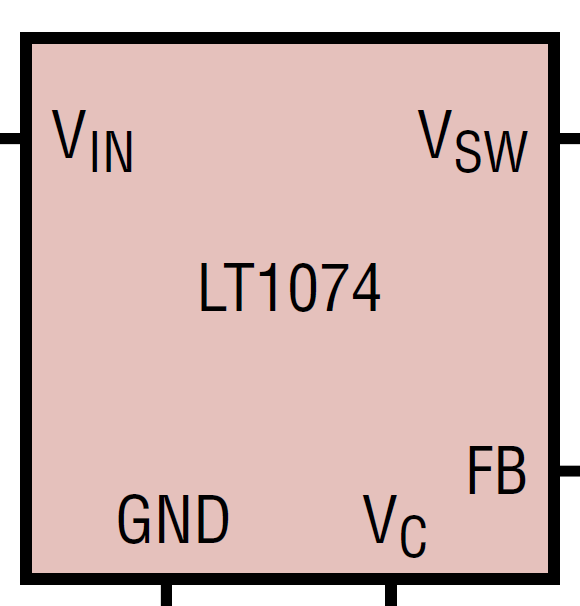
\includegraphics[width=0.2\textwidth]{LTData}%
\caption{Blockschaltbild des LT1074}
\label{fig::LTData}
\end{figure}

Die Schaltung wurde zunächst in LT-Spice simuliert und danach auf einer Lochrasterplatine aufgebaut:

\begin{figure}[h]
\centering
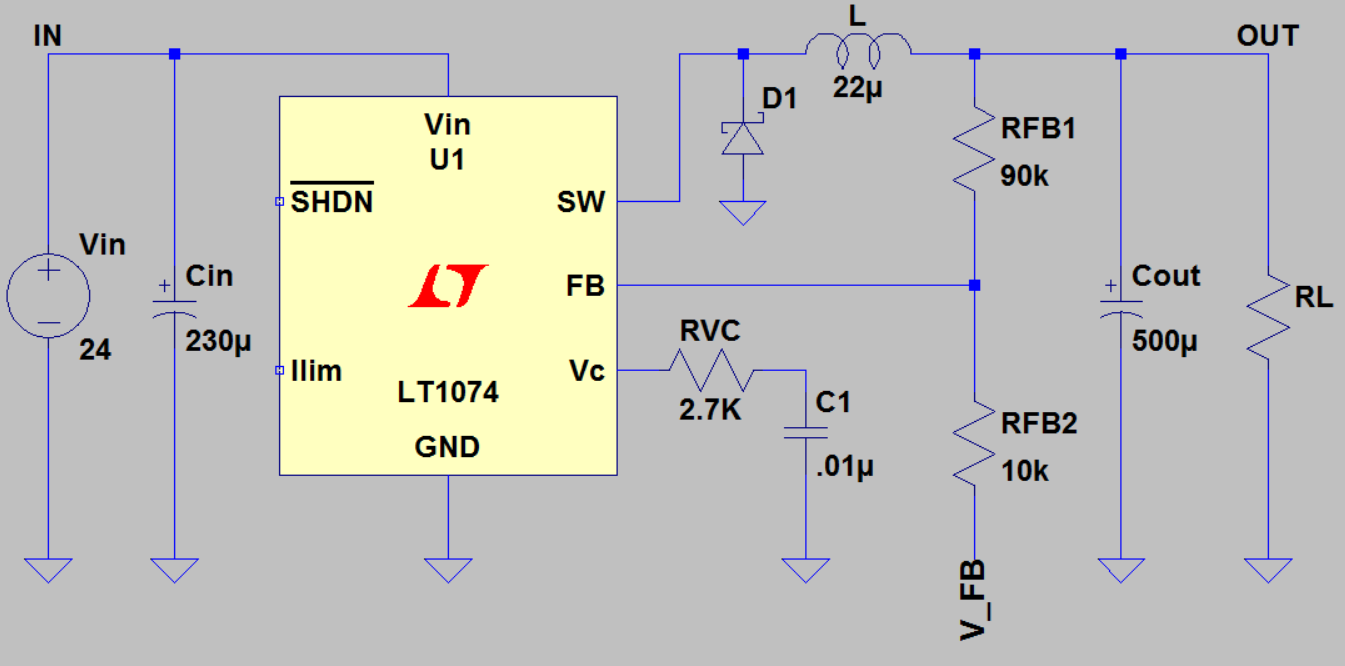
\includegraphics[width=0.8\textwidth]{LTSchemata}%
\caption{Beschaltung des Schaltreglers}%
\label{fig::LTSchemata}%
\end{figure}

Der Widerstand RFB1 wurde nach der folgenden Fromel berechnet:

\[
R_{FB1}=\frac{R_{FB2}\cdot V_{Outmax}}{2.21V}-R_{FB2}
\]

Dabei sind $V_{Outmax} =22$V und $R_{FB2} =10$k$\Omega$, dies ergibt für $R_{FB1} \approx 90$k$\Omega$

Die Spule sowie die Kondensatoren und der Widerstand $R_{Vc}$ wurden gemäss der Appplication Note von Linear Technologies dimensioniert und entsprechen den Empfehlungen des Herstellers.

Mittels der Spannung $V_{FB}$ kann nun die Ausgangsspannung folgendermassen verändert werden:

\[
V_{FB}=2.21\text{V}\cdot\frac{R_{FB1}+R_{FB2}}{R_{FB1}}-V_{out}\cdot\frac{R_{FB2}}{R_{FB1}}
\]

Man sieht sofort das bei einer $V_{FB}$ Spannung von 0V die Spannung maximal wird, das Maximum am Ausgang wird mit einer Spannung von 2.46V erreicht. 

Die Funktion dieser Schaltung wurde im Kapitel \ref{subsec:ValRegler} getestet und validiert.
\end{document}






\subsection{Bedienung}
Die Bedienung wurde für eine übersichtliche und schnelle Anwendung einfach gehalten. Auf der Vorderseite hat es drei Tasten und ein vierzeiliges LCD-Display mit je 16 Charakter für die visuelle Darstellung. Die Tasten sind jeweils aktiv High am Mikrocontroller angeschlossen mittels einem Taster-Pull-Up-Schaltkreis, zu sehen in Abbildung \ref{fig:SwitchPullUp_Software}. Der Pull-Up Widerstand hat einen Wert von $10k\Omega$, der mit einem Taster auf Erde verbunden wird.

\begin{figure}[h]
	\centering
		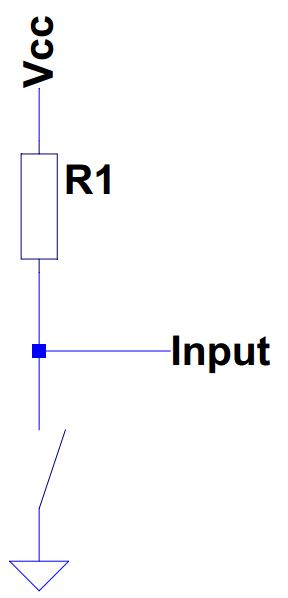
\includegraphics[width=0.15\textwidth]{Taster.jpg}
	\caption{Taster-Pull-Up-Schaltkreis}
	\label{fig:SwitchPullUp_Software}
\end{figure}

Die Taster wurden mit einer Softwarelösung entprellt, ansonsten konnte keine genaue Einstellung der Bestrahlungsstärke erreicht werden, da die Feder im Taster beim Drücken ein undeutliches Signal erzeugt und so ein exaktes und regelmässiges Zählen unmöglich macht. Wird ein Taster betätigt, wird der Widerstand und der Pin des Mikrokontrollers auf Masse verbunden und am Mikrokontroller entsteht ein Low-Zustand, also eine logische Null. Der Tasterzustand wird dann mit der Software ausgelesen.

Das Display stammt von Midas und ist die visuelle Schnittstelle zum Benutzer. Das LCD ist im vier Bit Modus an den Mikrocontroller angeschlossen. Die restlichen Kontakte und der Lesen-Schreiben-Anschluss (Read-Write-Pin) wurden auf Erde verbunden. Der LCD wird mit 5 Volt über den eingebauten DC-DC-Wandler versorgt.
\section{Software}

\subsection{Regelung}
\subsection{Bedienung}
Die Software zur Bedienung wurde in drei Teile gestaltet. Hardwaremäßig wurde nur das geringste an Elementen verwendet. Die drei Bedienelemente sind jeweils Aktiv High am Mikrocontroller geschaltet mittels einem Taster-Pull-Up-Schaltkreis \ref{fig:SwitchPullUp_Software}. Der Pull-Up Widerstand ist $10k\Omega$, der mit einem Taster auf Erde verbunden wird.

\begin{figure}[h]
	\centering
		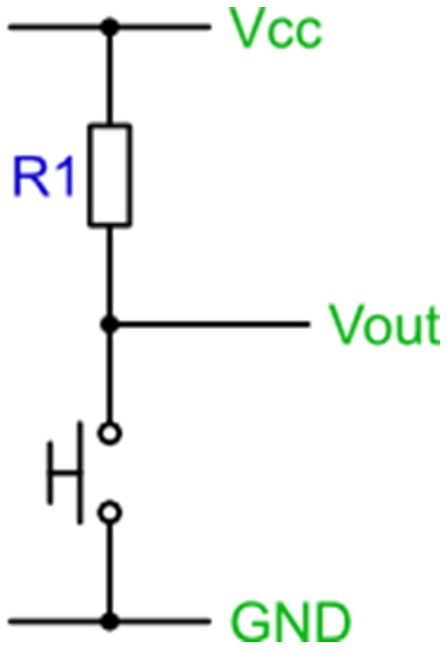
\includegraphics[width=0.25\textwidth]{switchpullupcircuit.jpg}
	\caption{Taster-Pull-Up-Schaltkreis}
	\label{fig:SwitchPullUp_Software}
\end{figure}


%ISR (TIMER0_OVF_vect)
Der Timer-Interrupt im Mikrocontroller ruft alle 16ms eine Funktion auf, die den Taster entprellt, aber auch die Länge des Tasterzustandes registriert.
%button |= ~old_button & current_button & BUTTONMASK;
Der Taster (button) wird als gedrückt erkannt, wenn die Inverse vom alten Zustand (old\_button), dem momentanen Zustand (current\_button) und der Pinmaske (BUTTONMASK)übereinstimmen.
%if (button)
Die folgende If-Bedingung zählt den Bestrahlungswert hoch. Einmal tippen zählt den Bestrahlungswert um eins hoch. Der Wertebereich liegt zwischen 20 und 100. Eine weitere If-Bedingung setzt den Bestrahlungswert beim überschreiten von 100 (Wert grösser gleich 101) zurück auf 20. In dieser sowie in der anderen Bedingung wird das automatische Zählen (autorepeat) auf 50, als Verzögerung, gesetzt.
Der gleiche Code wurde für das Abwärtzählen geschrieben mit dem Unterschied, dass eine Bedingung die Nicht-Zehnerzahlen erkennt und auf die nächst kleinere Zehnerzahl dekrementiert. Würde nämlich die Zahl 55, die ein Integer ist, durch Zehn dividiert mit Zehn multipliziert und um Zehn verringert werden, 40 ergeben.
In der Else-Bedingung wird zunächst geprüft, ob der Taster immer noch gedrückt wird (current\_button and BUTTONMASK). Ist die Bedingung erfüllt, dekrementiert die Funktion einen Wert, der den Unterschied zwischen Tippen und Drücken macht. Bei Null ist die Bedingung erfüllt und der Bestrahlungswert wird um zehn erhöht. Dabei springt er nur auf die nächste Zehnerzahl (Bestrahlungswert gleich Bestrahlungswert geteilt durch 10 multipliziert mit 10 und addiert mit 10). Hier wird wieder darauf geachtet, dass die Zahl 101 nicht überschreitet, sonst wird sie auf 20 zurückgesetzt.
Abgeschlossen wird die Funktion mit dem setzen vom alten Zustand gleich zum neuen Zustand.
Der Bestrahlungswert wird nach der Funktion in eine Variable gespeichert und auf dem Display angezeigt.
\newline
\subsection{Software}
\section{Validierung}

\subsection{Hardware}
\section{Schlusswort}

Virtual-Sun konnte nicht erfolgreich abgeschlossen werden. Die theoretischen Grundlagen bezüglich der Ausgangskennlinie, sowie der verschmutzten und der defekten Solarzelle sind vorhanden. Des weiteren sind diese Kennlinien bereits in der Software umgesetzt worden. Der Schaltregler konnte bis auf den Kurzschlussfall in Betrieb genommen werden und auch die Ausgabe der momentanen Spannungs- Stromwerte ist möglich. Buttons?

Die folgenden Bereiche konnten jedoch nicht in einen funktionsfähigen Betriebszustand gebracht werden: Die Ansteuerung des DA-Wandlers, sowie die Messung des Regler Ausganges. Diese beiden Schaltungsteile wurden in der Theorie konzipiert und dimensioniert, konnten jedoch aufgrund Zeitmangels nicht mehr in Betrieb genommen werden, 

\begin{appendix}
\section{Verifizierung Messaufbau}

\subsection{Spannungsmessung}\label{subsec_messu}
Die Spannung wird mittels eines Spannungsteilers aus zwei Widerstände bemessen. Die Toleranz beider Widerstände beträgt $\pm$ 1\%, im schlechtesten Fall ist ein Widerstand am oberen Ende der Toleranz, der andere am unteren Ende (beispielsweise 39.39k$\Omega$ und 9.9k$\Omega$ anstelle von 39k$\Omega$ und 10k$\Omega$). Der maximal mögliche Fehler beträgt damit 2.02\%. \newline
Um diesen Fehler auszuschliessen, wurde die Spannung am Ausgang des Spannungsteilers bei der grössten und der kleinsten möglichen Ausgangsspannung gemessen und die Differenz als 202.3mV pro V Ausgangsspannungserhöhung bestimmt. Mit den in Tabelle \ref{tab:messU} folgenden Messreihe wurde die Genauigkeit dieser Schaltung verifiziert.
\begin{table}
\centering
\begin{tabular}{|r|r|r|r|}
	\hline
	\textbf{Ausgangsspannung} & \textbf{Messwert $messU$} & \textbf{Differenz} & \textbf{Fehler} \\ \hline
	0.0V & 0mV & - & 0.0mV \\ \hline
	1.0V & 202mV & 202mV & -0.3mV \\ \hline
	2.0V & 406mV & 204mV & +1.7mV \\ \hline
	3.0V & 608mV & 202mV & -0.3mV \\ \hline
	4.0V & 811mV & 203mV & +0.7mV \\ \hline
	5.0V & 1013mV & 202mV & -0.3mV \\ \hline
	6.0V & 1216mV & 203mV & +0.7mV \\ \hline
	7.0V & 1418mV & 202mV & -0.3mV \\ \hline
	8.0V & 1621mV & 203mV & +0.7mV \\ \hline
	9.0V & 1824mV & 203mV & +0.7mV \\ \hline
	10.0V & 2026mV & 202mV & -0.3mV \\ \hline
	11.0V & 2228mV & 202mV & -0.3mV \\ \hline
	12.0V & 2430mV & 202mV & -0.3mV \\ \hline
	13.0V & 2632mV & 202mV & -0.3mV \\ \hline
	14.0V & 2834mV & 202mV & -0.3mV \\ \hline
	15.0V & 3036mV & 202mV & -0.3mV \\ \hline
	16.0V & 3239mV & 203mV & +0.7mV \\ \hline
	17.0V & 3441mV & 202mV & -0.3mV \\ \hline
	18.0V & 3644mV & 203mV & +0.7mV \\ \hline
	19.0V & 3845mV & 201mV & -1.3mV \\ \hline
	20.0V & 4048mV & 203mV & +0.7mV \\ \hline
	21.0V & 4251mV & 203mV & +0.7mV \\ \hline
	22.0V & 4454mV & 203mV & +0.7mV \\ \hline
	23.0V & 4657mV & 203mV & +0.7mV \\ \hline
	24.0V & 4860mV & 203mV & +0.7mV \\ \hline
\end{tabular}
\caption{Verifizierung der Messwerte $messU$ des Spannungsteilers.}
\label{tab:messU}
\end{table}
Die Fehler sind sehr klein und gleichen sich zumeist aus. Ausserdem sind die Fehler jeweils deutlich kleiner als die Auflösung des AD-Wandlers des Mikrocontrollers. Die Ausgangsspannung beträgt gemäss obiger Messreihe:
\begin{equation}
	U=\text{Messwert}\cdot 4.938
\label{eq:messreihe_messu}
\end{equation}
Für die Software, in welcher alle Werte in Millivolt betrachtet werden, wird $istU$ mit Formel \ref{eq:messreihe_messu} folgendermassen bestimmt:
\begin{equation}
	istU=messU\cdot\frac{400}{81}
\label{eq:messreihe_messu_sw}
\end{equation}


\subsection{Strommessung}\label{subsec_messi}
Die Strommessung beinhaltet Widerstände, Operationsverstärker sowie einen Hallsensor, die allesamt Toleranzen unterworfen sind. Am kritischsten ist dabei sicherlich der Spannungsteiler aus 2x 1k$\Omega$, der für die Subtraktionsschaltung benötigt wird. Bei einer Toleranz von 1\% kann die Spannung dabei 2.5V$\pm$50.5mV betragen. Diese Spannungsdifferenz wird jedoch ebenfalls um den Faktor 7.5 Verstärkt, wodurch der maximale Fehler bereits 378.8mV beträgt, was bei 10bit Auflösung des AD-Wandlers durchaus relevant ist. \newline
Aus diesem Grund wurde eine Messreihe durchgeführt. Dabei wurde die Spannung am Ausgang der Messschaltung zuerst bei minimalem und anschliessend bei maximalem Strom der verfügbaren Stromquelle gemessen. Pro 0.2A mehr Ausgangsstrom sollte die Spannung $messI$ gemäss dieser Messung um 281.5mV zunehmen, ausserdem ist ein Offset von 247mV vorhanden. Diese Werte wurden bis zu einem Maximalstrom von 3.0A in Tabelle \ref{tab:messI} ermittelt.
\begin{table}%
\centering
\begin{tabular}{|r|r|r|r|}
	\hline
	\textbf{Ausgangsstrom} & \textbf{Messwert $messI$} & \textbf{Differenz} & \textbf{Fehler} \\ \hline
	0.0A & 247mV & - & 247mV \\ \hline
	0.2A & 525mV & 278mV & -3.5mV \\ \hline
	0.4A & 809mV & 284mV & +2.5mV \\ \hline
	0.6A & 1093mV & 284mV & +2.5mV \\ \hline
	0.8A & 1374mV & 281mV & -0.5mV \\ \hline
	1.0A & 1660mV & 286mV & +4.5mV \\ \hline
	1.2A & 1943mV & 283mV & +1.5mV \\ \hline
	1.4A & 2223mV & 280mV & -1.5mV \\ \hline
	1.6A & 2507mV & 284mV & +2.5mV \\ \hline
	1.8A & 2785mV & 278mV & -3.5mV \\ \hline
	2.0A & 3061mV & 276mV & -5.5mV \\ \hline
	2.2A & 3344mV & 283mV & +1.5mV \\ \hline
	2.4A & 3629mV & 285mV & +3.5mV \\ \hline
	2.6A & 3907mV & 278mV & -3.5mV \\ \hline
	2.8A & 4187mV & 280mV & -1.5mV \\ \hline
	3.0A & 4469mV & 282mV & +0.5mV \\ \hline
\end{tabular}
\caption{Verifizierung der Messwerte $messI$ der Strommessung.}
\label{tab:messI}
\end{table}
Die Fehler sind ungefähr gleichmässig verteilt und können mit der Ungenauigkeit der verwendeten Stromquelle erklärt werden. Jedoch sind sie deutlich grösser als beim Spannungsteiler, jedoch noch weit unterhalb der geforderten Genauigkeit. Der Ausgangsstrom beträgt gemäss obiger Messreihe:
\begin{equation}
	I=\frac{Messwert-247mV}{1.407}
\label{eq:messreihe_messi}
\end{equation}
Für die Software, in welcher alle Werte in Millivolt und Milliampere betrachtet werden, wird $istI$ mit Formel \ref{eq:messreihe_messi} folgendermassen bestimmt:
\begin{equation}
	istI=\left(messI-247mV\right)\cdot\frac{4222}{3}
\label{eq:messreihe_messi_sw}
\end{equation}


\newpage
\section{CD-ROM}
\end{appendix}

\end{document}